
%% bare_jrnl.tex
%% V1.3
%% 2007/01/11
%% by Michael Shell
%% see http://www.michaelshell.org/
%% for current contact information.
%%
%% This is a skeleton file demonstrating the use of IEEEtran.cls
%% (requires IEEEtran.cls version 1.7 or later) with an IEEE journal paper.
%%
%% Support sites:
%% http://www.michaelshell.org/tex/ieeetran/
%% http://www.ctan.org/tex-archive/macros/latex/contrib/IEEEtran/
%% and
%% http://www.ieee.org/



% *** Authors should verify (and, if needed, correct) their LaTeX system  ***
% *** with the testflow diagnostic prior to trusting their LaTeX platform ***
% *** with production work. IEEE's font choices can trigger bugs that do  ***
% *** not appear when using other class files.                            ***
% The testflow support page is at:
% http://www.michaelshell.org/tex/testflow/


%%*************************************************************************
%% Legal Notice:
%% This code is offered as-is without any warranty either expressed or
%% implied; without even the implied warranty of MERCHANTABILITY or
%% FITNESS FOR A PARTICULAR PURPOSE! 
%% User assumes all risk.
%% In no event shall IEEE or any contributor to this code be liable for
%% any damages or losses, including, but not limited to, incidental,
%% consequential, or any other damages, resulting from the use or misuse
%% of any information contained here.
%%
%% All comments are the opinions of their respective authors and are not
%% necessarily endorsed by the IEEE.
%%
%% This work is distributed under the LaTeX Project Public License (LPPL)
%% ( http://www.latex-project.org/ ) version 1.3, and may be freely used,
%% distributed and modified. A copy of the LPPL, version 1.3, is included
%% in the base LaTeX documentation of all distributions of LaTeX released
%% 2003/12/01 or later.
%% Retain all contribution notices and credits.
%% ** Modified files should be clearly indicated as such, including  **
%% ** renaming them and changing author support contact information. **
%%
%% File list of work: IEEEtran.cls, IEEEtran_HOWTO.pdf, bare_adv.tex,
%%                    bare_conf.tex, bare_jrnl.tex, bare_jrnl_compsoc.tex
%%*************************************************************************

% Note that the a4paper option is mainly intended so that authors in
% countries using A4 can easily print to A4 and see how their papers will
% look in print - the typesetting of the document will not typically be
% affected with changes in paper size (but the bottom and side margins will).
% Use the testflow package mentioned above to verify correct handling of
% both paper sizes by the user's LaTeX system.
%
% Also note that the "draftcls" or "draftclsnofoot", not "draft", option
% should be used if it is desired that the figures are to be displayed in
% draft mode.
%
\documentclass[journal]{IEEEtran}
%
% If IEEEtran.cls has not been installed into the LaTeX system files,
% manually specify the path to it like:
% \documentclass[journal]{../sty/IEEEtran}





% Some very useful LaTeX packages include:
% (uncomment the ones you want to load)


% *** MISC UTILITY PACKAGES ***
%
%\usepackage{ifpdf}
% Heiko Oberdiek's ifpdf.sty is very useful if you need conditional
% compilation based on whether the output is pdf or dvi.
% usage:
% \ifpdf
%   % pdf code
% \else
%   % dvi code
% \fi
% The latest version of ifpdf.sty can be obtained from:
% http://www.ctan.org/tex-archive/macros/latex/contrib/oberdiek/
% Also, note that IEEEtran.cls V1.7 and later provides a builtin
% \ifCLASSINFOpdf conditional that works the same way.
% When switching from latex to pdflatex and vice-versa, the compiler may
% have to be run twice to clear warning/error messages.






% *** CITATION PACKAGES ***
%
%\usepackage{cite}
% cite.sty was written by Donald Arseneau
% V1.6 and later of IEEEtran pre-defines the format of the cite.sty package
% \cite{} output to follow that of IEEE. Loading the cite package will
% result in citation numbers being automatically sorted and properly
% "compressed/ranged". e.g., [1], [9], [2], [7], [5], [6] without using
% cite.sty will become [1], [2], [5]--[7], [9] using cite.sty. cite.sty's
% \cite will automatically add leading space, if needed. Use cite.sty's
% noadjust option (cite.sty V3.8 and later) if you want to turn this off.
% cite.sty is already installed on most LaTeX systems. Be sure and use
% version 4.0 (2003-05-27) and later if using hyperref.sty. cite.sty does
% not currently provide for hyperlinked citations.
% The latest version can be obtained at:
% http://www.ctan.org/tex-archive/macros/latex/contrib/cite/
% The documentation is contained in the cite.sty file itself.






% *** GRAPHICS RELATED PACKAGES ***
%
\ifCLASSINFOpdf
  \usepackage[pdftex]{graphicx}
  % declare the path(s) where your graphic files are
  % graphicspath{{../pdf/}{../jpeg/}}
  % and their extensions so you won't have to specify these with
  % every instance of \includegraphics
  \DeclareGraphicsExtensions{.pdf,.jpeg,.png}
\else
  % or other class option (dvipsone, dvipdf, if not using dvips). graphicx
  % will default to the driver specified in the system graphics.cfg if no
  % driver is specified.
  % \usepackage[dvips]{graphicx}
  % declare the path(s) where your graphic files are
  % \graphicspath{{../eps/}}
  % and their extensions so you won't have to specify these with
  % every instance of \includegraphics
  % \DeclareGraphicsExtensions{.eps}
\fi
% graphicx was written by David Carlisle and Sebastian Rahtz. It is
% required if you want graphics, photos, etc. graphicx.sty is already
% installed on most LaTeX systems. The latest version and documentation can
% be obtained at: 
% http://www.ctan.org/tex-archive/macros/latex/required/graphics/
% Another good source of documentation is "Using Imported Graphics in
% LaTeX2e" by Keith Reckdahl which can be found as epslatex.ps or
% epslatex.pdf at: http://www.ctan.org/tex-archive/info/
%
% latex, and pdflatex in dvi mode, support graphics in encapsulated
% postscript (.eps) format. pdflatex in pdf mode supports graphics
% in .pdf, .jpeg, .png and .mps (metapost) formats. Users should ensure
% that all non-photo figures use a vector format (.eps, .pdf, .mps) and
% not a bitmapped formats (.jpeg, .png). IEEE frowns on bitmapped formats
% which can result in "jaggedy"/blurry rendering of lines and letters as
% well as large increases in file sizes.
%
% You can find documentation about the pdfTeX application at:
% http://www.tug.org/applications/pdftex





% *** MATH PACKAGES ***
%
%\usepackage[cmex10]{amsmath}
% A popular package from the American Mathematical Society that provides
% many useful and powerful commands for dealing with mathematics. If using
% it, be sure to load this package with the cmex10 option to ensure that
% only type 1 fonts will utilized at all point sizes. Without this option,
% it is possible that some math symbols, particularly those within
% footnotes, will be rendered in bitmap form which will result in a
% document that can not be IEEE Xplore compliant!
%
% Also, note that the amsmath package sets \interdisplaylinepenalty to 10000
% thus preventing page breaks from occurring within multiline equations. Use:
%\interdisplaylinepenalty=2500
% after loading amsmath to restore such page breaks as IEEEtran.cls normally
% does. amsmath.sty is already installed on most LaTeX systems. The latest
% version and documentation can be obtained at:
% http://www.ctan.org/tex-archive/macros/latex/required/amslatex/math/





% *** SPECIALIZED LIST PACKAGES ***
%
%\usepackage{algorithmic}
% algorithmic.sty was written by Peter Williams and Rogerio Brito.
% This package provides an algorithmic environment fo describing algorithms.
% You can use the algorithmic environment in-text or within a figure
% environment to provide for a floating algorithm. Do NOT use the algorithm
% floating environment provided by algorithm.sty (by the same authors) or
% algorithm2e.sty (by Christophe Fiorio) as IEEE does not use dedicated
% algorithm float types and packages that provide these will not provide
% correct IEEE style captions. The latest version and documentation of
% algorithmic.sty can be obtained at:
% http://www.ctan.org/tex-archive/macros/latex/contrib/algorithms/
% There is also a support site at:
% http://algorithms.berlios.de/index.html
% Also of interest may be the (relatively newer and more customizable)
% algorithmicx.sty package by Szasz Janos:
% http://www.ctan.org/tex-archive/macros/latex/contrib/algorithmicx/




% *** ALIGNMENT PACKAGES ***
%
%\usepackage{array}
% Frank Mittelbach's and David Carlisle's array.sty patches and improves
% the standard LaTeX2e array and tabular environments to provide better
% appearance and additional user controls. As the default LaTeX2e table
% generation code is lacking to the point of almost being broken with
% respect to the quality of the end results, all users are strongly
% advised to use an enhanced (at the very least that provided by array.sty)
% set of table tools. array.sty is already installed on most systems. The
% latest version and documentation can be obtained at:
% http://www.ctan.org/tex-archive/macros/latex/required/tools/


%\usepackage{mdwmath}
%\usepackage{mdwtab}
% Also highly recommended is Mark Wooding's extremely powerful MDW tools,
% especially mdwmath.sty and mdwtab.sty which are used to format equations
% and tables, respectively. The MDWtools set is already installed on most
% LaTeX systems. The lastest version and documentation is available at:
% http://www.ctan.org/tex-archive/macros/latex/contrib/mdwtools/


% IEEEtran contains the IEEEeqnarray family of commands that can be used to
% generate multiline equations as well as matrices, tables, etc., of high
% quality.


%\usepackage{eqparbox}
% Also of notable interest is Scott Pakin's eqparbox package for creating
% (automatically sized) equal width boxes - aka "natural width parboxes".
% Available at:
% http://www.ctan.org/tex-archive/macros/latex/contrib/eqparbox/





% *** SUBFIGURE PACKAGES ***
%\usepackage[tight,footnotesize]{subfigure}
% subfigure.sty was written by Steven Douglas Cochran. This package makes it
% easy to put subfigures in your figures. e.g., "Figure 1a and 1b". For IEEE
% work, it is a good idea to load it with the tight package option to reduce
% the amount of white space around the subfigures. subfigure.sty is already
% installed on most LaTeX systems. The latest version and documentation can
% be obtained at:
% http://www.ctan.org/tex-archive/obsolete/macros/latex/contrib/subfigure/
% subfigure.sty has been superceeded by subfig.sty.



%\usepackage[caption=false]{caption}
%\usepackage[font=footnotesize]{subfig}
% subfig.sty, also written by Steven Douglas Cochran, is the modern
% replacement for subfigure.sty. However, subfig.sty requires and
% automatically loads Axel Sommerfeldt's caption.sty which will override
% IEEEtran.cls handling of captions and this will result in nonIEEE style
% figure/table captions. To prevent this problem, be sure and preload
% caption.sty with its "caption=false" package option. This is will preserve
% IEEEtran.cls handing of captions. Version 1.3 (2005/06/28) and later 
% (recommended due to many improvements over 1.2) of subfig.sty supports
% the caption=false option directly:
%\usepackage[caption=false,font=footnotesize]{subfig}
%
% The latest version and documentation can be obtained at:
% http://www.ctan.org/tex-archive/macros/latex/contrib/subfig/
% The latest version and documentation of caption.sty can be obtained at:
% http://www.ctan.org/tex-archive/macros/latex/contrib/caption/




% *** FLOAT PACKAGES ***
%
%\usepackage{fixltx2e}
% fixltx2e, the successor to the earlier fix2col.sty, was written by
% Frank Mittelbach and David Carlisle. This package corrects a few problems
% in the LaTeX2e kernel, the most notable of which is that in current
% LaTeX2e releases, the ordering of single and double column floats is not
% guaranteed to be preserved. Thus, an unpatched LaTeX2e can allow a
% single column figure to be placed prior to an earlier double column
% figure. The latest version and documentation can be found at:
% http://www.ctan.org/tex-archive/macros/latex/base/



%\usepackage{stfloats}
% stfloats.sty was written by Sigitas Tolusis. This package gives LaTeX2e
% the ability to do double column floats at the bottom of the page as well
% as the top. (e.g., "\begin{figure*}[!b]" is not normally possible in
% LaTeX2e). It also provides a command:
%\fnbelowfloat
% to enable the placement of footnotes below bottom floats (the standard
% LaTeX2e kernel puts them above bottom floats). This is an invasive package
% which rewrites many portions of the LaTeX2e float routines. It may not work
% with other packages that modify the LaTeX2e float routines. The latest
% version and documentation can be obtained at:
% http://www.ctan.org/tex-archive/macros/latex/contrib/sttools/
% Documentation is contained in the stfloats.sty comments as well as in the
% presfull.pdf file. Do not use the stfloats baselinefloat ability as IEEE
% does not allow \baselineskip to stretch. Authors submitting work to the
% IEEE should note that IEEE rarely uses double column equations and
% that authors should try to avoid such use. Do not be tempted to use the
% cuted.sty or midfloat.sty packages (also by Sigitas Tolusis) as IEEE does
% not format its papers in such ways.


%\ifCLASSOPTIONcaptionsoff
%  \usepackage[nomarkers]{endfloat}
% \let\MYoriglatexcaption\caption
% \renewcommand{\caption}[2][\relax]{\MYoriglatexcaption[#2]{#2}}
%\fi
% endfloat.sty was written by James Darrell McCauley and Jeff Goldberg.
% This package may be useful when used in conjunction with IEEEtran.cls'
% captionsoff option. Some IEEE journals/societies require that submissions
% have lists of figures/tables at the end of the paper and that
% figures/tables without any captions are placed on a page by themselves at
% the end of the document. If needed, the draftcls IEEEtran class option or
% \CLASSINPUTbaselinestretch interface can be used to increase the line
% spacing as well. Be sure and use the nomarkers option of endfloat to
% prevent endfloat from "marking" where the figures would have been placed
% in the text. The two hack lines of code above are a slight modification of
% that suggested by in the endfloat docs (section 8.3.1) to ensure that
% the full captions always appear in the list of figures/tables - even if
% the user used the short optional argument of \caption[]{}.
% IEEE papers do not typically make use of \caption[]'s optional argument,
% so this should not be an issue. A similar trick can be used to disable
% captions of packages such as subfig.sty that lack options to turn off
% the subcaptions:
% For subfig.sty:
% \let\MYorigsubfloat\subfloat
% \renewcommand{\subfloat}[2][\relax]{\MYorigsubfloat[]{#2}}
% For subfigure.sty:
% \let\MYorigsubfigure\subfigure
% \renewcommand{\subfigure}[2][\relax]{\MYorigsubfigure[]{#2}}
% However, the above trick will not work if both optional arguments of
% the \subfloat/subfig command are used. Furthermore, there needs to be a
% description of each subfigure *somewhere* and endfloat does not add
% subfigure captions to its list of figures. Thus, the best approach is to
% avoid the use of subfigure captions (many IEEE journals avoid them anyway)
% and instead reference/explain all the subfigures within the main caption.
% The latest version of endfloat.sty and its documentation can obtained at:
% http://www.ctan.org/tex-archive/macros/latex/contrib/endfloat/
%
% The IEEEtran \ifCLASSOPTIONcaptionsoff conditional can also be used
% later in the document, say, to conditionally put the References on a 
% page by themselves.





% *** PDF, URL AND HYPERLINK PACKAGES ***
%
\usepackage{url}
\usepackage{hyperref}
% url.sty was written by Donald Arseneau. It provides better support for
% handling and breaking URLs. url.sty is already installed on most LaTeX
% systems. The latest version can be obtained at:
% http://www.ctan.org/tex-archive/macros/latex/contrib/misc/
% Read the url.sty source comments for usage information. Basically,
% \url{my_url_here}.


% Listings
\usepackage{listings}

\lstdefinelanguage{HTML5}{}

% *** Do not adjust lengths that control margins, column widths, etc. ***
% *** Do not use packages that alter fonts (such as pslatex).         ***
% There should be no need to do such things with IEEEtran.cls V1.6 and later.
% (Unless specifically asked to do so by the journal or conference you plan
% to submit to, of course. )


% correct bad hyphenation here
\hyphenation{op-tical net-works semi-conduc-tor}


\begin{document}
\lstset{language=HTML}  

%
% paper title
% can use linebreaks \\ within to get better formatting as desired
\title{Viability of HTML5 video as a replacement for plug-in based approaches of delivering video content to user agents}
%
%
% author names and IEEE memberships
% note positions of commas and nonbreaking spaces ( ~ ) LaTeX will not break
% a structure at a ~ so this keeps an author's name from being broken across
% two lines.
% use \thanks{} to gain access to the first footnote area
% a separate \thanks must be used for each paragraph as LaTeX2e's \thanks
% was not built to handle multiple paragraphs
%

%\author{Michael~Shell,~\IEEEmembership{Member,~IEEE,}
%        John~Doe,~\IEEEmembership{Fellow,~OSA,}
%        and~Jane~Doe,~\IEEEmembership{Life~Fellow,~IEEE}% <-this % stops a space
\author{David~Hulme%
\thanks{K. Martinez is with the Department
of Electronics and Computer Science, University of Southampton, UK e-mail: (see http://users.ecs.soton.ac.uk/km).}}% <-this % stops a space
%\thanks{J. Doe and J. Doe are with Anonymous University.}% <-this % stops a space
%\thanks{Manuscript received April 19, 2005; revised January 11, 2007.}}

% note the % following the last \IEEEmembership and also \thanks - 
% these prevent an unwanted space from occurring between the last author name
% and the end of the author line. i.e., if you had this:
% 
% \author{....lastname \thanks{...} \thanks{...} }
%                     ^------------^------------^----Do not want these spaces!
%
% a space would be appended to the last name and could cause every name on that
% line to be shifted left slightly. This is one of those "LaTeX things". For
% instance, "\textbf{A} \textbf{B}" will typeset as "A B" not "AB". To get
% "AB" then you have to do: "\textbf{A}\textbf{B}"
% \thanks is no different in this regard, so shield the last } of each \thanks
% that ends a line with a % and do not let a space in before the next \thanks.
% Spaces after \IEEEmembership other than the last one are OK (and needed) as
% you are supposed to have spaces between the names. For what it is worth,
% this is a minor point as most people would not even notice if the said evil
% space somehow managed to creep in.



% The paper headers
%\markboth{Journal of \LaTeX\ Class Files,~Vol.~6, No.~1, January~2007}%
%{Shell \MakeLowercase{\textit{et al.}}: Bare Demo of IEEEtran.cls for Journals}
% The only time the second header will appear is for the odd numbered pages
% after the title page when using the twoside option.
% 
% *** Note that you probably will NOT want to include the author's ***
% *** name in the headers of peer review papers.                   ***
% You can use \ifCLASSOPTIONpeerreview for conditional compilation here if
% you desire.




% If you want to put a publisher's ID mark on the page you can do it like
% this:
%\IEEEpubid{0000--0000/00\$00.00~\copyright~2007 IEEE}
% Remember, if you use this you must call \IEEEpubidadjcol in the second
% column for its text to clear the IEEEpubid mark.



% use for special paper notices
%\IEEEspecialpapernotice{(Invited Paper)}




% make the title area
\maketitle


\begin{abstract}
%\boldmath
HTML5 defines a method for videos to be embedded directly into a web page. The ability to directly embed videos into web pages removes the web browser's dependence on third party software and opens up new possibilities for the integration of video multimedia with other web content.

However, for any new web technology to gain acceptance it must be comparable to the current technology in use. In this paper, an examination of the viability of HTML5 video as a replacement for the current plug-in based technologies in use is conducted as well as research into the new opportunities it can provide.
\end{abstract}

\IEEEpeerreviewmaketitle

\section{Introduction}
\IEEEPARstart{I}{nternet} video traffic is growing. Cisco predict that by 2017, consumer Internet video traffic will account for 69\% of all consumer Internet traffic \cite{website:ciscoForecastAndMethodology}. In addition, nearly half of all Internet traffic will originate from a non-PC device \cite{website:ciscoForecastAndMethodology}. It is therefore important to ensure that technologies are in place to deliver this content to users and provide a high quality viewing experience across a wide range of devices and platforms.

Multimedia is accessed via a user agent: software acting on behalf of a user. A typical scenario could consist of a browser as the user agent, with video embedded on a web page. Historically this has been achieved through the use of third party plug-ins such as Adobe Flash\footnote{Adobe Flash Player: \url{http://www.adobe.com/uk/software/flash/about/}}, henceforth referred to in this paper as Flash, or Microsoft Silverlight\footnote{Microsoft Silverlight: \url{http://www.microsoft.com/silverlight/}}, henceforth referred to as Silverlight. Flash was well on the way to becoming the de facto standard for embedding video into web pages \cite{article:HTML5LeadsAWebRevolution}. However, in 2010 Apple announced that they would not allow Flash on their mobile devices, citing as concerns the closed nature, reliability, security and performance of Flash \cite{website:appleFlash}. Watanabe et al. also raised concerns regarding the security of Flash \cite{inproceedings:flashSecurity}. An industry agreed standard addressing these concerns is required.

HTML5, an emerging specification from the W3C, includes a definition for a video element. This element enables videos to be embedded directly into a web page \cite{standard:html5}. Natively embedding videos into web pages removes the web browser's dependence on a third party plug-in, thus increasing openness. In addition it allows the web browser to handle the video content in any manner it wishes, leading to an enhanced experience across different devices. Finally, it opens new possibilities for the integration of video multimedia with other web content.

However, any replacement for embedding video content must be suitable and comparable to the current technology in use. Each user agent that supports HTML5 video may implement the specification slightly differently, which may lead to inconsistent support for all features. This paper will research key areas relating to the delivery of video content to user agents and the subsequent user interaction with the video, to examine whether HTML5 video is a viable replacement for the current plug-in based technologies in use.

\section{Content Delivery}
In this section different aspects of delivering video content to user agents will be investigated.

\subsection{Embedding Method} 
HTML specifies the \textless object\textgreater~tag which allows for external resources to be embedded in a web page. The `type' attribute tells the web browser the Internet media type of the content, allowing the browser to choose an appropriate plug-in to display the content \cite{standard:html5}. As Daoust et al. noted, ``relying on third-party plug-ins to render the video works fine in a variety of use cases'' \cite{article:towardsVideoOnTheWebWithHTML5}. However, they also stated that because the video is rendered in a black box, from the browser's perspective, CSS and SVG cannot be used to style the video or apply visual effects \cite{article:towardsVideoOnTheWebWithHTML5}. Problems can also be encountered if the user agent cannot find an appropriate plug-in to handle the object.

The \textless video\textgreater~tag, new to HTML5, directly integrates the video into the browser, alleviating these problems. By indicating to the user agent that video content is embedded, they are able to decide how to display the content. For example, on iOS devices a place holder is presented and when selected launches a full screen player \cite{website:safariHTML5}.

\begin{figure}[!t]
\centering
\includegraphics[width=3.5in]{chrooma-approach}
\caption{Dynamic video overlays in HTML5 \cite{inproceedings:theChroomaApproach}}
\label{fig:chroomaApproach}
\end{figure} 

In addition, the embedding of video content using the \textless video\textgreater~tag opens up opportunities for developers. For example, Oehme et al. added dynamic overlays to a video, with related data from various Internet sources, see Figure \ref{fig:chroomaApproach} \cite{inproceedings:theChroomaApproach}.

The HTML5 \textless canvas\textgreater~tag gives developers a resolution-dependent bitmap canvas to which visual images can be rendered \cite{standard:html5}. The \textless canvas\textgreater~tag can be used in conjunction with the \textless video\textgreater~tag to produce engaging applications, such as the work of Fulton, S. and Fulton, J. who describe a canvas video puzzle application, or Quax et al. who used a hidden video element to receive a video stream before manipulating the video and then displaying on a canvas element \cite{book:html5canvas}\cite{inproceedings:aPracticalAndScableMethodForStreaming}.

\subsection{Supported Formats}
An important distinction to make is the difference between video containers, codecs and formats. A codec is the way in which the audio or video is encoded, for example H.264, Theora, VP6, VP8 and Spark. A container describes the structure of the file and which codecs are in use \cite{website:videoFormatsGuide}. Some example containers include MP4, WebM, Ogg, AVI and FLV. A format is the combination of a container and codecs, for example an MP4 container with the H.264 video codec and MP3 audio codec.

Flash only plays videos contained within the FLV (Flash Video) container or the ShockWave Flash container used in earlier releases \cite{article:flashPlayer}. Flash supports the VP6 and Spark codecs and since version 9, supports H.264 \cite{article:flashPlayer}\cite{website:flashSupportedFormats}. Silverlight supports the ASF, MP4 and 3GP containers and supports a variety of codecs including H.264 and WMV \cite{website:silverlightSupportedFormats}.

HTML5 does not specify support for any specific codec or container format, leading to different codecs and containers being supported by different user agents \cite{article:towardsVideoOnTheWebWithHTML5}. The three codecs and containers most widely supported are H.264 in an MP4 container, Theora in an Ogg container and VP8 in a WebM container \cite{article:towardsVideoOnTheWebWithHTML5}.

Table \ref{tab:supportedCodecsAndContainers} shows the support for these three formats across different browsers. It is important to note that Table \ref{tab:supportedCodecsAndContainers} only considers that a format is supported if it is supported natively by the browser, for example Firefox relies on a Flash fall back to play H.264 content \cite{website:firefoxVideoMobileAndTheOpenWeb}.

\begin{table}
	\caption{Supported Codecs and Containers by Browser \cite{inproceedings:applicationOfHTML5Multimedia}\cite{article:towardsVideoOnTheWebWithHTML5}}
	\label{tab:supportedCodecsAndContainers}
	\centering
  \begin{tabular}{|l|l|l|l|}
    \hline
    \textbf{Browser}    & \textbf{H.264 in MP4} & \textbf{Theora in Ogg} & \textbf{VP8 in WebM} \\ \hline
    IE8        & No           & No            & No          \\ \hline
    IE9+       & Yes          & No            & No          \\ \hline
    Chrome 18+ & Yes          & Yes           & Yes         \\ \hline
    Firefox 6+ & No           & Yes           & Yes         \\ \hline
    Opera 12+  & No           & Yes           & Yes         \\ \hline
    Safari 5+  & Yes          & No            & No          \\ \hline
  \end{tabular}
\end{table}

Table \ref{tab:supportedCodecsAndContainers} illustrates how there is inconsistent support for different formats across browsers, often caused by patents and licensing fees. For example, H.264 is not royalty free and although VP8 and Theora have been released with royalty-free licences, Intellectual Property Rights holders may appear in the future \cite{article:towardsVideoOnTheWebWithHTML5}\cite{website:theoraBenefits}. To ensure that a video is playable across multiple browsers, developers can specify multiple \textless source\textgreater~tags within the \textless video\textgreater~tag that specify different formats of the video that are available. The browser is then able to choose to play the format it prefers. An example of this is shown in Figure \ref{lst:HTML5VideoExample}. If the browser does not support HTML5 video then the \textless object\textgreater~tag, which embeds a Flash video, will be rendered instead.

\begin{figure}
\caption{HTML5 Video Example}
\label{lst:HTML5VideoExample}
\begin{lstlisting}[frame=single,language=HTML5,basicstyle=\footnotesize]
<video>
 <source src="video.mp4"
   type='video/mp4; codecs="avc1.4D401E, mp4a.40.2"'>
 <source src="video.ogg"
   type='video/ogg; codecs="theora, vorbis"'>
 <source src="video.webm"
   type='video/webm; codecs="vp8.0, vorbis"'>
 <object>
  <param name="movie" value="video.flv">
 </object>
</video>
\end{lstlisting}
\end{figure}

\subsection{Delivery Methods}
There are two distinct approaches for delivering video content to clients. The first is traditional streaming through protocols such as Real Time Streaming Protocol (RTSP)\footnote{RFC 2326: \url{http://www.ietf.org/rfc/rfc2326.txt}} with Real-time Transport Protocol (RTP)\footnote{RFC 3550: \url{http://www.ietf.org/rfc/rfc3550.txt}} or Adobe's Real Time Message Protocol (RTMP)\footnote{Real-Time Messaging Protocol (RTMP) specification: \url{http://www.adobe.com/devnet/rtmp.html}} \cite{article:areWeInTheMiddleOfAVideoStreamingRevolution}. These are push-based streaming protocols where the server streams packets to the client until the client interrupts or stops the session \cite{article:watchingVideoOverTheWeb}. The streamed packets are not cached on the client \cite{article:watchingVideoOverTheWeb}. A media server is required to manage the streams, an approach traditionally used by Flash \cite{article:flashPlayer}.

The second is pulled-based approaches, usually over the HTTP protocol. Delivering over HTTP allows Content Delivery Networks (CDNs) to be used which can improve caching, efficiency and reduce licensing costs \cite{article:towardsVideoOnTheWebWithHTML5}\cite{inproceedings:HTTPAsTheNarrowWaist}. In addition, HTTP traffic can traverse firewalls and Network Address Translation (NAT) more simply than other transport protocols. %citation? could use several, not sure of the best one

Progressive download is the simplest HTTP streaming approach. The client begins downloading the video and starts to play it when a minimum threshold has been reached \cite{article:watchingVideoOverTheWeb}. However there are two problems with this approach: firstly, the client is unable to jump to a point in the video that has not downloaded and secondly there is no guarantee that the delivery rate will remain constant, which could lead to unwanted latency \cite{article:towardsVideoOnTheWebWithHTML5}. %is latency the right word? % could mention http range requests, see 'to chunk or not to chunk', but not that important

To enable skipping to any point in the video, the stream can be divided into chunks, or fragments, to be independently requested by the client \cite{article:areWeInTheMiddleOfAVideoStreamingRevolution}. Apple's HTTP Live Streaming (HLS)\footnote{HTTP Live Streaming: \url{http://tools.ietf.org/html/draft-pantos-http-live-streaming-12}} and Microsoft's Smooth Streaming\footnote{Microsoft Smooth Streaming: \url{http://www.iis.net/downloads/microsoft/smooth-streaming}} are example protocols that use this technique \cite{article:watchingVideoOverTheWeb}. Smooth Streaming contains all the fragments in a single MP4 file as shown in Figure \ref{fig:mp4Structure} \cite{article:watchingVideoOverTheWeb}. The MFRA index box shown in Figure \ref{fig:mp4Structure} allows easy and accurate seeking within the file \cite{website:smoothStreamingArchitecture}. HLS uses a different approach and stores each media fragment in a separate file \cite{article:watchingVideoOverTheWeb}.

\begin{figure}[!t]
\centering
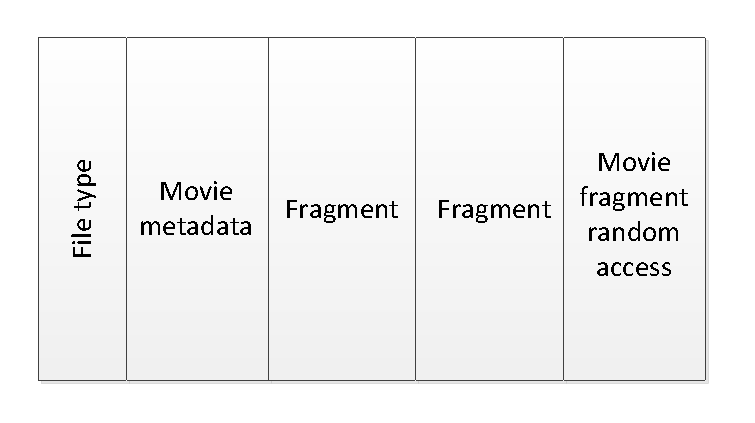
\includegraphics[width=3.5in]{smooth-streaming}
\caption{Fragmented MP4 file format structure, adapted from \cite{website:smoothStreamingArchitecture}}
\label{fig:mp4Structure}
\end{figure} 

These protocols also provide adaptive streaming. Between segment requests, the client can assess the current network conditions and switch between different bit rates of the same media, based on the optimal bit rate achievable \cite{article:areWeInTheMiddleOfAVideoStreamingRevolution}.

In order to function, these techniques rely on the delivery of a manifest file to the client to determine which URIs should be requested. % citation?
Support therefore requires a specific plug-in, Silverlight in the case of Smooth Streaming, or support for the technology built into the HTML5 video implementation \cite{inproceedings:aSeamlessIntegrationOfAdaptiveHTTPStreaming}. % could cite 'a seamless integration of ...' which says that HLS is only supported on apple products, although this is now not quite true

\begin{figure}[!t]
\centering
\includegraphics[width=2.5in]{dash-procedure2}
\caption{DASH media retrieval procedure, adapted from  \cite{inproceedings:dynamicAdapativeHTTPStreamingLive}}
\label{fig:dashProcedure}
\end{figure} 

Dynamic Adaptive Streaming over HTTP (DASH)\footnote{Dynamic
adaptive streaming over HTTP (DASH) ISO/IEC 23009-1} is an international standard developed by the Moving Picture Expert Group (MPEG) in order to provide an alternative to proprietary protocols such as HLS and Smooth Streaming. To play video content over DASH, a client first obtains a manifest file in the form of an Media Presentation Description (MPD) \cite{article:MPEGDASH}. Using this data, the client selects the appropriate encoded file and segment before requesting over HTTP \cite{article:MPEGDASH}. The first segment requested should have a low bit rate to allow for streaming to begin quickly \cite{inproceedings:dynamicAdapativeHTTPStreamingLive}. Between segment requests, the requested quality level can change. Figure \ref{fig:dashProcedure} shows the operation of a DASH session.

Rainer et al. describe a way to use DASH in combination with the HTML5 video element by utilising Media Source Extensions (MSE)\footnote{Media Source Extensions (MSE): \url{http://www.w3.org/TR/media-source/}} which allow JavaScript to construct media streams for the HTML5 audio and video elements \cite{standard:mse} \cite{inproceedings:aSeamlessIntegrationOfAdaptiveHTTPStreaming}. However, currently MSE is only supported on Chrome and Firefox, so as yet it is not a complete solution \cite{website:mdnMediaSource}.

Plug-in based approaches use both push and pull based streaming methods. Flash uses push based RTMP, whilst Silverlight uses pull based Smooth Streaming. HTML5 video does not declare which streaming protocols implementations should support. Typically, HTTP streaming is supported using a variety of techniques, as opposed to traditional streaming protocols such as RTP, which are not envisioned as the main streaming methods for HTML5 \cite{article:towardsVideoOnTheWebWithHTML5}.

\subsection{Delivery Classes}
There are two classes of media that can be delivered to clients: on-demand media and live media \cite{techreport:aReviewOfHTTPLiveStreaming}. On-demand media has been previously recorded and encoded, whilst live media is captured, compressed and transmitted on the fly, thus requiring significant computing resources \cite{techreport:aReviewOfHTTPLiveStreaming}. Any technology used to embed video in web pages should support the delivery of both these media types.

Plug-in based approaches such as Flash are capable of streaming live video to user agents through Adobe's Flash Media Server (FMS) using RTMP \cite{techreport:aReviewOfHTTPLiveStreaming}. However, these technologies have difficulties traversing firewalls and NAT and require dedicated network infrastructure \cite{inproceedings:dynamicAdapativeHTTPStreamingLive}. % may not be the best citation

An example of a very simple video streaming solution for HTML5 is to set up an HTTP stream from VLC media player\footnote{VLC media player: \url{http://www.videolan.org/vlc/}}. The web browser makes a single HTTP request for the stream and once buffered it can begin playing. However, this approach requires a continuous connection between client and server and does not account for changes in the connection speed. More sophisticated live streaming solutions can be provided by HLS or DASH, leveraging existing CDNs to distribute content \cite{techreport:aReviewOfHTTPLiveStreaming} \cite{inproceedings:dynamicAdapativeHTTPStreamingLive}. 

\begin{figure}[!t]
\centering
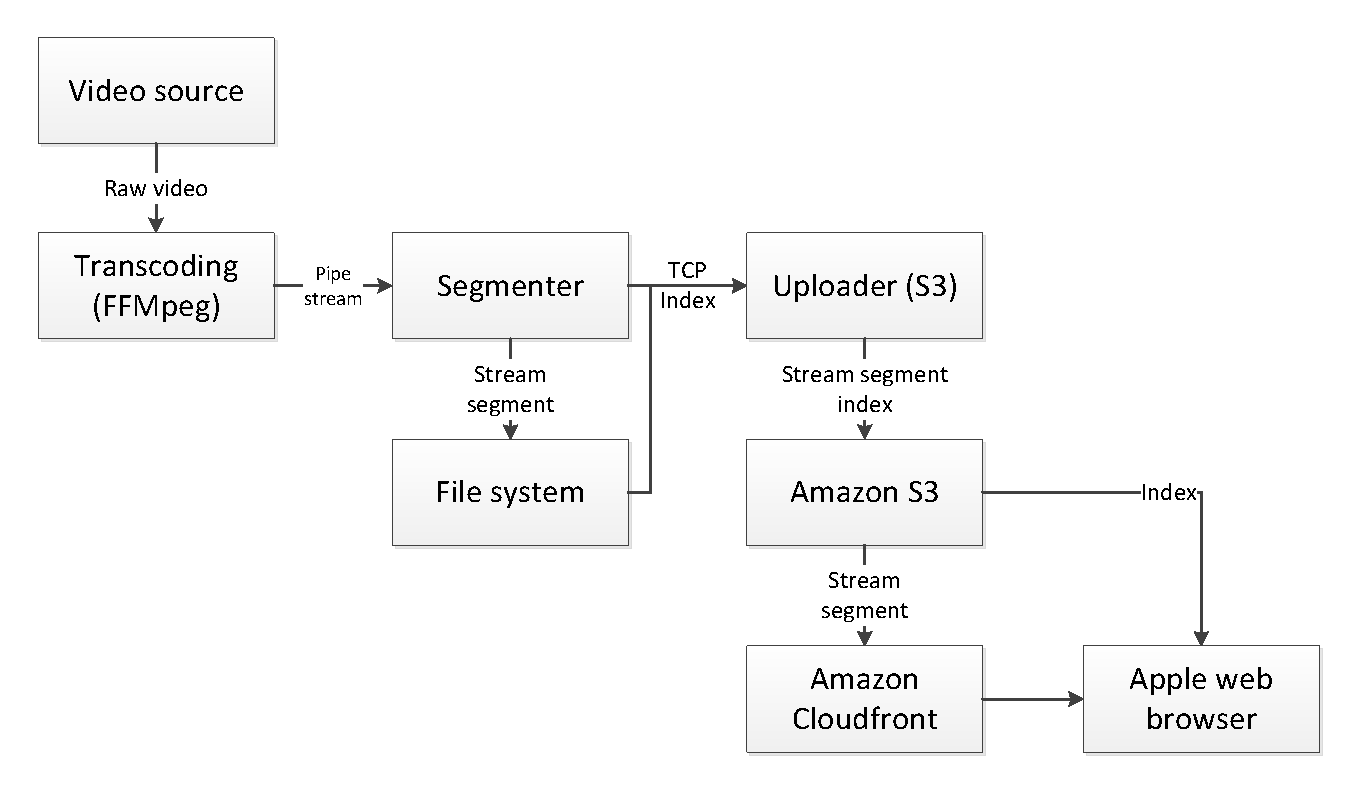
\includegraphics[width=3.5in]{streaming-diagram}
\caption{HLS using Amazon services architecture \cite{website:iPhoneHLSAmazon}}
\label{fig:hlsAmazonArch}
\end{figure} 

\begin{figure}[!t]
\centering
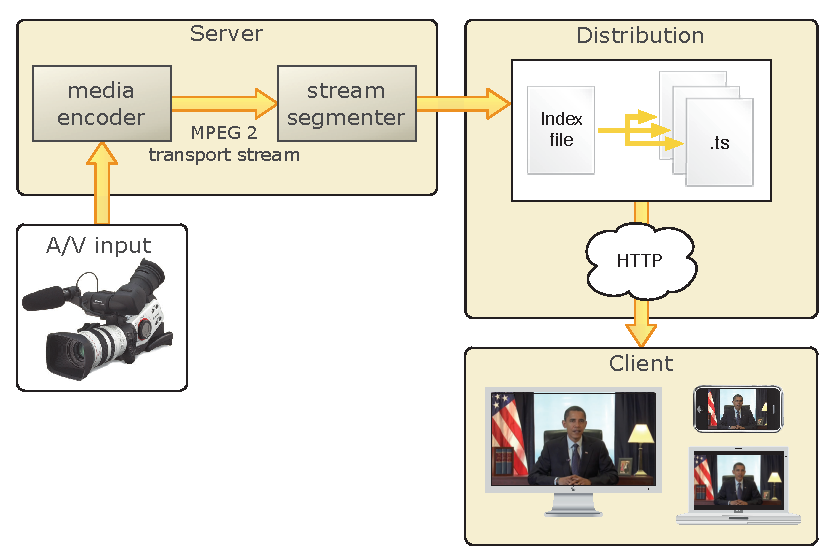
\includegraphics[width=3.5in]{streaming-architecture}
\caption{Live streaming over HTTP architecture, adapted from  \cite{techreport:aReviewOfHTTPLiveStreaming}}
\label{fig:HTTPLiveStreamingArch}
\end{figure}

Fecheyr-Lippens noted that Akamai, the world's leading CDN, has a specific solution for delivering video to iOS devices using HLS \cite{whitePaper:akamaiHDNetwork}\cite{techreport:aReviewOfHTTPLiveStreaming}. He also described McDonald's work of setting up HLS through Amazon services \cite{website:iPhoneHLSAmazon}. McDonald's architecture for delivering live video content to Apple user agents is shown in Figure \ref{fig:hlsAmazonArch}. He calculated the cost and concluded that for 100 streams of 5 minutes worth of video, it would cost about 20 cents for the use of Amazon services \cite{website:iPhoneHLSAmazon}. A generalised architecture for live streaming over HTTP is shown in Figure \ref{fig:HTTPLiveStreamingArch}.

\subsection{Content Protection}
All video content that is delivered to user agents is vulnerable to the `analogue hole'. At some point in the delivery chain there must be an analogue component, be it a loud speaker or video display, in order for a user to digest the content \cite{inproceedings:closingTheAnalogueHole}. At this point the analogue signals can be recorded, digitised and redistributed, thus bypassing any content protection measures that have been put in place \cite{inproceedings:closingTheAnalogueHole}.

However, since this capturing process may require specialist equipment and can take a large amount of time, the average user will want to access the file in its original digital form. Therefore content protection systems should focus on encrypting the digital file and occluding its location.

All videos delivered over HTTP progressive download will have the video file accessible at some URI. In HTML5 the location of the original video file can be found by examining the `src' attribute, see Figure \ref{lst:HTML5VideoExample}. For plug-in based approaches such as Flash, tools can be used to discover the URI.

This approach can be made more difficult for the client by including a one-time token in the URI. For example, the URI could be \texttt{http://example.com/video?id=1\&token=12345}. Valid tokens can be stored in a database on the server and removed once they have been requested. When a web page containing a video loads, the video will be automatically requested. If a user attempts to request the video again, in order to save it, the server can throw an error.

The second approach for capturing streamed media is through examining the browser cache. All video content delivered via HTTP streaming methods is cached by the browser. The cached video data can be then extracted using tools such as VideoCacheView\footnote{VideoCacheView by Nir Sofer: \url{http://www.nirsoft.net/utils/video_cache_view.html}}. Using this tool, a test to capture a video from YouTube was successful.

Whilst content delivered over traditional streaming protocols such as RTMP is not cached, it is possible to capture the stream from the browser and save to a file using tools such as RTMPDumpHelper\footnote{RTMPDumpHelper by Nir Sofer: \url{http://www.nirsoft.net/utils/rtmp_dump_helper.html}}. Content providers can make this technique more difficult by preventing unauthorised clients from accessing the video stream using technologies such as Adobe's SWF Verification\footnote{SWF verification for Protected HTTP Dynamic Streaming: \url{http://www.adobe.com/devnet/adobe-media-server/articles/swf-verification-protected-http-dynamic-streaming.html}}. 

Adobe also offers encrypted RTMP and Flash Access, a solution that sits between the Flash player and the browser to protect streamed content \cite{whitePaper:flashAccess}.
% could talk more about flash access if we need to

If a user obtains the original file, Digital Rights Management (DRM) technologies such as Microsoft's Windows Media DRM\footnote{Binding digital content to a portable storage device or the like in a DRM system: \url{http://www.google.com/patents/US7010808}} or Apple's FairPlay can be used to control or prevent playback.

HTML5 does not specify a DRM system \cite{article:HTML5LeadsAWebRevolution}. However in September 2013, Tim Berners-Lee approved supporting the playback of protected content as part of the HTML Working Group's charter\footnote{HTML Working Group Charter: \url{http://www.w3.org/2013/09/html-charter.html}} culminating in the Encrypted Media Extensions (EME) draft\footnote{Encrypted Media Extensions: \url{https://dvcs.w3.org/hg/html-media/raw-file/tip/encrypted-media/encrypted-media.html}} \cite{email:newHTMLCharter}. EME provides a common API to interact with DRM systems to control the playback of protected content \cite{standard:eme}. Whilst some were critical of including EME in the charter, API extensions to HTML media are in the scope of the group, thus so is EME \cite{website:EEFDRM}\cite{email:emeInScope}. In addition, it is important to provide a framework for DRM technologies to gain support for HTML5 video from content providers.

DRM systems are supported by HLS and DASH. DASH allows the resource to specify which DRM systems it supports in the MPD, enabling the content to be encrypted once and streamed to clients that support different DRM systems \cite{article:MPEGDASH}. HLS allows for individual encryption of segments using AES-128 encryption \cite{techreport:aReviewOfHTTPLiveStreaming}.

\section{Performance}
Globally, it is predicted that mobile data traffic will increase 13-fold between 2012 and 2017 \cite{website:ciscoForecastAndMethodology}. This will lead to an increasing amount of Internet video being consumed on mobile devices. Such devices are less powerful than a typical desktop computer and  have a strong emphasis on optimising their battery life. It is therefore important that watching HTML5 video uses the device's resources effectively and efficiently. % could probably say this better.

Ilias et al. conducted a study to analyse the video streaming performance between Flash video and HTML5 video on low-power laptops \cite{inproceedings:aStudyOfVideoPerformanceAnalysis}. They looked at two video performance metrics, frame rate and CPU usage, whilst streaming a video over wired and wireless networks across a variety of browsers. Their study showed that the implementation of HTML5 video in each browser had a significant effect on the performance. This can be seen in Figure \ref{fig:cpuPerformanceGraph}. Overall the average CPU for Flash was 77\% and 87\% for HTML5 video. This shows that on average, HTML5 video requires 13\% more CPU power than Flash. In addition, in IE9 HTML5 video used 95\% of the CPU. This certainly has the potential to cause playback problems on mobile devices and cause frustration to users. However, the HTML5 video result for Chrome suggests that the CPU usage is heavily influenced by the HTML5 video implementation. Thus as the implementations are developed over time, the situation should improve.

A test was conducted to compare the performance of playing a Flash and HTML5 video from YouTube in Google Chrome. YouTube provides the option to use either the Flash or HTML5 player. Out of the three major browsers, only Google Chrome supports both YouTube's Flash and HTML5 players. Over several tests, Flash averaged 58\% CPU usage, whilst HTML5 averaged 53\% CPU utilisation. From these results, it is reasonable to say that HTML5 video is a viable replacement for Flash to deliver YouTube content to the browser. 

\begin{figure}[!t]
\centering
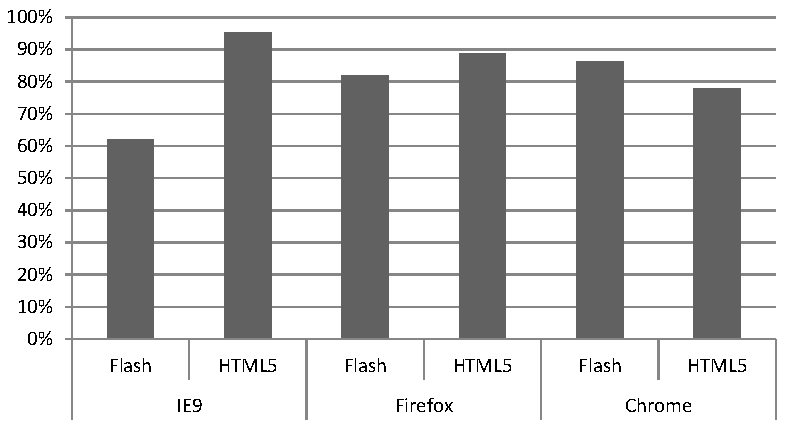
\includegraphics[width=3.5in]{cpu-performance-graph}
\caption{CPU usage across different browsers on low-power laptops. Data produced by averaging results from Ilias et al. \cite{inproceedings:aStudyOfVideoPerformanceAnalysis} across two different CPU monitoring tools and both wired and wireless networks.}
\label{fig:cpuPerformanceGraph}
\end{figure} 

\section{Accessibility}
Accessibility on the web is governed by the W3C 2008 recommendation, Web Content Accessibility Guidelines (WCAG)\footnote{Web Content Accessibility Guidelines (WCAG) 2.0: \url{http://www.w3.org/TR/WCAG20/}}. More recently, the User Agent Accessibility Guidelines (UAAG), a standard to provide additional advice on the application user interface, is in development \cite{website:implementingUAAG}.

Moreno et al. propose three areas that must be considered to deliver accessible multimedia content: accessible video, accessible web page and accessible user interaction \cite{article:disablityStandardsForMultimediaOnTheWeb}.

\subsection{Accessible Video}
WCAG 2.0 Guideline 1.2 requires that developers provide alternatives for time-based media such as alternative text, captions, audio description and sign language as shown in Table \ref{tab:wcag2Guidelines} \cite{standard:wcag2}.

\begin{table}
  \caption{WCAG 2.0 Guidelines \cite{standard:wcag2}}
  \label{tab:wcag2Guidelines}
  	\centering
    \begin{tabular}{|l|l|p{1.5cm}|}
    \hline
    \textbf{Guideline}          & \textbf{Type} & \textbf{Conformance level} \\ \hline
    1.1.1 Non-text Content                 & All         & A                 \\ \hline
    1.2.1 Alternative for time-based media & Prerecorded & A                 \\ \hline
    1.2.2 Captions                         & Prerecorded & A                 \\ \hline
    1.2.4 Captions                         & Live        & AA                \\ \hline
    1.2.5 Audio Description                & Prerecorded & AA                \\ \hline
    1.2.6 Sign Language                    & Prerecorded & AAA               \\ \hline
    \end{tabular}
\end{table}

The W3C provides documents detailing how these guidelines can be met for different technologies such as Flash\footnote{Flash Techniques for WCAG 2.0: \url{http://www.w3.org/TR/WCAG20-TECHS/flash.html}} and Silverlight\footnote{Silverlight Techniques for WCAG 2.0: \url{http://www.w3.org/TR/WCAG20-TECHS/silverlight.html}}. For example, the Flash document explains how developers can add subtitles to their Flash videos using an XML file to meet WCAG 2.0 Guideline 1.2.2 \cite{website:flashTechniquesForWCAG}.

Pfeiffer and Parker describe existing implementations for supporting subtitles for HTML5 video \cite{inproceedings:accessibilityForTheHTML5VideoElement}. They describe the work of Jan Gerber who used JavaScript to load subtitles from a text file and display them on screen in time with an HTML5 video\footnote{Jan Gerber, jquery.srt.js: \url{http://v2v.cc/~j/jquery.srt/}} \cite{inproceedings:accessibilityForTheHTML5VideoElement}.

HTML5 specifies a \textless track\textgreater~tag that can be used to specify timed text tracks for media elements \cite{standard:html5}. Figure \ref{lst:trackExample} shows the minimal mark-up required to include subtitles with a video. The subtitle track referenced in Figure \ref{lst:trackExample} is formatted using Web Video Text Track (WebVTT)\footnote{WebVTT: \url{http://dev.w3.org/html5/webvtt/}}, a new standard being developed by the W3C. Dutton said that the track element was available in Internet Explorer and Google Chrome \cite{website:html5RocksTrackElement}. A test was carried out to confirm this and found that whilst Google Chrome does support WebVTT subtitles, Internet Explorer 11 and Firefox do not. In June 2013, Wald et al. found that none of the browsers on mobile devices natively supported WebVTT \cite{article:synote}. However, by using the MediaElement.js player\footnote{MediaElement.js: \url{http://mediaelementjs.com/}}, WebVTT subtitles could be supported on the iPad \cite{article:synote}. WebVTT files can be included as part of an HLS stream, or delivered as part of a live DASH stream as demonstrated by Concolato and Le Feuvre \cite{misc:HTTPLiveStreaming}\cite{inproceedings:liveHTTPSubtitle}.

Instead of using an external text track file, data can be embedded within container formats such as Ogg \cite{inproceedings:accessibilityForTheHTML5VideoElement}\cite{website:oggSubtitles}. However, this is not the approach recommended by the W3C. %citation?

Testing was carried out using the widely used JAWS\footnote{JAWS: \url{http://www.freedomscientific.com/products/fs/jaws-product-page.asp}} screen reader. A YouTube video with captions\footnote{YouTube Captions and Subtitles video: \url{https://www.youtube.com/watch?v=QRS8MkLhQmM}} was played using both the YouTube HTML5 and Flash players. JAWS was easily able to detect the controls and subtitles when the HTML5 player was used, but could not when the Flash player was used. A test was also carried out to see if JAWS could automatically detect subtitles when using the \textless track\textgreater~tag in Google Chrome; it could not.

In conclusion, HTML5 video can be accessible, although cross-browser native support for video subtitles is some way off.

\begin{figure}
\caption{HTML5 Track Example \cite{website:html5RocksTrackElement}}
\begin{lstlisting}[frame=single,language=HTML5]
<video>
  <source src="video.mp4">
  <track src="subtitles.vtt"
    label="English subtitles"
     kind="subtitles" srclang="en">
  </track>
</video>
\end{lstlisting}
\label{lst:trackExample}
\end{figure}

\subsection{Accessible Web Page}
Accessibility must be considered when including media on a web page. If a link is provided to a video it must meet certain criteria described in WCAG 2.0 Guideline 4.1.2. If it is embedded, there any no relevant WCAG 2.0 guidelines.

\subsection{Accessible User Interaction}
WCAG 2.0 Guideline 2.2.2 states that for any moving content, there must exist some mechanism to pause the content. Most video embedding solutions provide this. Guideline 2.1.1 states that all content must be operable through the keyboard \cite{standard:wcag2}. One of the key problems with plug-in based approaches such as Flash or Silverlight is that any video playback controls are generally inaccessible to screen readers which read web pages based on HTML tags \cite{inproceedings:transformingFlashToXML}\cite{incollection:accessibilityEvaluationForMultimediaContent}. Plug-in content is delivered in a binary format and determining the structure of the content at runtime is near impossible \cite{inproceedings:transformingFlashToXML}.

Adobe has provided a document, ``Best Practices for Accessible Flash Design'' which describes how Flash content can be understood by screen readers through Microsoft Active Accessibility\footnote{Microsoft Active Accessibility: \url{http://msdn.microsoft.com/en-us/library/windows/desktop/dd373592(v=vs.85).aspx
}} (MSAA) \cite{whitePaper:bestPracticesForAccessibleFlashDesign}. If an author of Flash content adds the required accessibility information into the content, Flash can expose their content to screen readers \cite{inproceedings:automaticAccesibilityTranscodingForFlashContent}.

% maybe I try and duplicate their findings?
However there are some limitations with this system. Flash exposes information about buttons even if the button has no active behaviour. Sato et al. found that the MSAA information for the Flash YouTube player states that there are 13 buttons in the player, where in fact there are only 5 shown to users. Some of the 13 buttons had no functional content and others had no keyboard access and so were inaccessible to blind users \cite{inproceedings:automaticAccesibilityTranscodingForFlashContent}.

% could talk about the survey in 'accessibility evaluation for multiemedia content'. but this was a while ago, so may not be relevant anymore?

In HTML5, default video controls can be included using the `controls' attribute on the \textless video\textgreater~tag. However, each web browser implements these controls differently and does not necessarily allow them to be controlled via the keyboard. Therefore, the default controls do not meet accessibility guidelines. Moreno et al. developed an accessible HTML5 video player by adding HTML buttons to control the video player which can be controlled by a screen reader \cite{incollection:html5SupportForAnAccessibleWeb}.

In conclusion, accessible environments are most easily achieved through the use of HTML pages created according to Web content accessibility guidelines \cite{incollection:accessibilityEvaluationForMultimediaContent}.

\section{Discussion}
In this paper, the viability of HTML5 video as a replacement for plug-in based approaches of delivering video has been examined, focussing on the areas of content delivery, performance and accessibility.

\subsection{Content Delivery}
Firstly, the method of embedding video media into a web page was discussed. Plug-in based approaches use the \textless object\textgreater~tag, whilst HTML5 video uses the \textless video\textgreater~tag. Using HTML5 video prevents the browser from relying on third party plug-ins and enables a viewing experience that is customised to that device. The \textless video\textgreater~tag also allows for richer integration and interaction with the browser through APIs, providing new opportunities for developers.

Secondly, this paper examined the video formats supported by HTML5 video and plug-in based approaches. Plug-in based approaches typically support a consistent set of formats across a variety of different platforms. The formats supported by HTML5 video differ between implementations, with no single format gaining universal support. This requires content providers to provide duplicates of the video in multiple formats to ensure cross-browser support.

Thirdly, the methods of content delivery were considered. Both HTML5 video and plug-in based approaches support adaptive streaming techniques of live and pre-recorded media, with HTML5 video favouring pull-based HTTP approaches and plug-in based approaches typically using push-based methods using RTMP and the like. Streaming technologies are built into plug-ins, whilst HTLM5 video requires user agent support. These streaming technologies can be implemented by the user agent itself, or in JavaScript through the MSE API. Using MSE means that user agents do not need to concern themselves with supporting streaming methods. However, MSE is not currently supported by all browsers.

Lastly, content protection was investigated. Plug-in based approaches have been used for years by content providers to deliver video content to user agents and many techniques exist to make capturing the streamed video very difficult and deliver an encrypted stream. HTML5 video does not specify any DRM methods, although it was agreed recently that an API to support these would be developed by the HTML5 W3C working group.

\subsection{Performance}
The performance of HTML5 video and plug-in based approaches was researched. It was found that although plug-in based approaches currently perform better, an impressive result for HTML5 video in Google Chrome suggests that as HTML5 video implementations improve, so will their performance. 

\subsection{Accessibility}
Both HTML5 video and plug-in based approaches can be made accessible, both in terms of the content they deliver and the interaction with the user agent. However, ensuring plug-in based approaches are accessible requires significant effort by developers, meaning accessibility is often not achieved. HTML5 video uses solely HTML elements, improving its accessible user interaction.

There are multiple methods of embedding subtitles in HTML5 media, improving upon the methods used by plug-in based approaches. However, there is work to be done to provide support for accessibility tools and across web browsers.

\section{Conclusion}
HTML5 video aims to create a more open web by not relying on third party plug-ins. It enables richer video applications to be developed and provides a customisable experience across platforms.

Currently there is no agreement on the formats that should be supported by HTML5 implementations, hindering the uptake of HTML5 video. Continued efforts need to be made to standardise this to give clarification to vendors and provide a consistent experience across user agents.

Through a variety of adaptive streaming methods, it is possible to deliver both live and pre-recorded content to users using HTML5 video in such a way that provides a good user experience. More work needs to be done to support MSE across browsers to ensure content can be delivered.

Content protection is addressed in HTML5 video through EME, however this is still in its infancy. Currently, Flash provides a more proven method of delivering protected content to users, so more work is required here to make HTML5 video viable for this purpose and convince distributors that their content can be suitably protected.

The performance of HTML5 video varies across user agents, however this should be addressed in the future.

Finally, HTML5 video increases the accessibility of video content on the web through its improved support for screen readers and closed captions.

In conclusion, HTML5 video is a viable replacement for plug-in based approaches, albeit with some work still to do. Technologies such as Flash, are more mature and currently offer a more consistent experience on desktop web browsers. In order for HTML5 to be considered viable, standardisation efforts must be continued. If they are successful, a standardised way of delivering video content to user agents will become a reality and it is hoped that the use of HTML5 video by content providers such as YouTube\footnote{YouTube HTML5: \url{https://www.youtube.com/html5}} will drive acceptance and lead to increased adoption.

% An example of a floating figure using the graphicx package.
% Note that \label must occur AFTER (or within) \caption.
% For figures, \caption should occur after the \includegraphics.
% Note that IEEEtran v1.7 and later has special internal code that
% is designed to preserve the operation of \label within \caption
% even when the captionsoff option is in effect. However, because
% of issues like this, it may be the safest practice to put all your
% \label just after \caption rather than within \caption{}.
%
% Reminder: the "draftcls" or "draftclsnofoot", not "draft", class
% option should be used if it is desired that the figures are to be
% displayed while in draft mode.
%
%\begin{figure}[!t]
%\centering
%\includegraphics[width=2.5in]{myfigure}
% where an .eps filename suffix will be assumed under latex, 
% and a .pdf suffix will be assumed for pdflatex; or what has been declared
% via \DeclareGraphicsExtensions.
%\caption{Simulation Results}
%\label{fig_sim}
%\end{figure}

% Note that IEEE typically puts floats only at the top, even when this
% results in a large percentage of a column being occupied by floats.


% An example of a double column floating figure using two subfigures.
% (The subfig.sty package must be loaded for this to work.)
% The subfigure \label commands are set within each subfloat command, the
% \label for the overall figure must come after \caption.
% \hfil must be used as a separator to get equal spacing.
% The subfigure.sty package works much the same way, except \subfigure is
% used instead of \subfloat.
%
%\begin{figure*}[!t]
%\centerline{\subfloat[Case I]\includegraphics[width=2.5in]{subfigcase1}%
%\label{fig_first_case}}
%\hfil
%\subfloat[Case II]{\includegraphics[width=2.5in]{subfigcase2}%
%\label{fig_second_case}}}
%\caption{Simulation results}
%\label{fig_sim}
%\end{figure*}
%
% Note that often IEEE papers with subfigures do not employ subfigure
% captions (using the optional argument to \subfloat), but instead will
% reference/describe all of them (a), (b), etc., within the main caption.


% An example of a floating table. Note that, for IEEE style tables, the 
% \caption command should come BEFORE the table. Table text will default to
% \footnotesize as IEEE normally uses this smaller font for tables.
% The \label must come after \caption as always.
%
%\begin{table}[!t]
%% increase table row spacing, adjust to taste
%\renewcommand{\arraystretch}{1.3}
% if using array.sty, it might be a good idea to tweak the value of
% \extrarowheight as needed to properly center the text within the cells
%\caption{An Example of a Table}
%\label{table_example}
%\centering
%% Some packages, such as MDW tools, offer better commands for making tables
%% than the plain LaTeX2e tabular which is used here.
%\begin{tabular}{|c||c|}
%\hline
%One & Two\\
%\hline
%Three & Four\\
%\hline
%\end{tabular}
%\end{table}


% Note that IEEE does not put floats in the very first column - or typically
% anywhere on the first page for that matter. Also, in-text middle ("here")
% positioning is not used. Most IEEE journals use top floats exclusively.
% Note that, LaTeX2e, unlike IEEE journals, places footnotes above bottom
% floats. This can be corrected via the \fnbelowfloat command of the
% stfloats package.


% if have a single appendix:
%\appendix[Proof of the Zonklar Equations]
% or
%\appendix  % for no appendix heading
% do not use \section anymore after \appendix, only \section*
% is possibly needed

% use appendices with more than one appendix
% then use \section to start each appendix
% you must declare a \section before using any
% \subsection or using \label (\appendices by itself
% starts a section numbered zero.)
%


\appendices
%\section{Proof of the First Zonklar Equation}
%Appendix one text goes here.

% you can choose not to have a title for an appendix
% if you want by leaving the argument blank
%\section{}
%Appendix two text goes here.


% use section* for acknowledgement
\section*{Acknowledgments}


The author would like to thank Dr. Kirk Martinez for his support and guidance.


% Can use something like this to put references on a page
% by themselves when using endfloat and the captionsoff option.
\ifCLASSOPTIONcaptionsoff
  \newpage
\fi



% trigger a \newpage just before the given reference
% number - used to balance the columns on the last page
% adjust value as needed - may need to be readjusted if
% the document is modified later
\IEEEtriggeratref{39}
% The "triggered" command can be changed if desired:
%\IEEEtriggercmd{\enlargethispage{-5in}}

% references section

% can use a bibliography generated by BibTeX as a .bbl file
% BibTeX documentation can be easily obtained at:
% http://www.ctan.org/tex-archive/biblio/bibtex/contrib/doc/
% The IEEEtran BibTeX style support page is at:
% http://www.michaelshell.org/tex/ieeetran/bibtex/
%\bibliographystyle{IEEEtran}
% argument is your BibTeX string definitions and bibliography database(s)
%\bibliography{IEEEabrv,../bib/paper}
%
% <OR> manually copy in the resultant .bbl file
% set second argument of \begin to the number of references
% (used to reserve space for the reference number labels box)
\bibliographystyle{IEEEtran}
\bibliography{report}


%\begin{thebibliography}{1}

%\bibitem{IEEEhowto:kopka}
%H.~Kopka and P.~W. Daly, \emph{A Guide to \LaTeX}, 3rd~ed.\hskip 1em plus
%  0.5em minus 0.4em\relax Harlow, England: Addison-Wesley, 1999.

%\end{thebibliography}

% biography section
% 
% If you have an EPS/PDF photo (graphicx package needed) extra braces are
% needed around the contents of the optional argument to biography to prevent
% the LaTeX parser from getting confused when it sees the complicated
% \includegraphics command within an optional argument. (You could create
% your own custom macro containing the \includegraphics command to make things
% simpler here.)
%\begin{biography}[{\includegraphics[width=1in,height=1.25in,clip,keepaspectratio]{mshell}}]{Michael Shell}
% or if you just want to reserve a space for a photo:

%\begin{IEEEbiography}{Michael Shell}
%Biography text here.
%\end{IEEEbiography}

% if you will not have a photo at all:
%\begin{IEEEbiographynophoto}{John Doe}
%Biography text here.
%\end{IEEEbiographynophoto}

% insert where needed to balance the two columns on the last page with
% biographies
%\newpage

%\begin{IEEEbiographynophoto}{Jane Doe}
%Biography text here.
%\end{IEEEbiographynophoto}

% You can push biographies down or up by placing
% a \vfill before or after them. The appropriate
% use of \vfill depends on what kind of text is
% on the last page and whether or not the columns
% are being equalized.

%\vfill

% Can be used to pull up biographies so that the bottom of the last one
% is flush with the other column.
%\enlargethispage{-5in}



% that's all folks
\end{document}


